\documentclass[aspectratio=169]{beamer}
\usetheme{Madrid}
\usecolortheme{default}

\usepackage{booktabs}
\usepackage{amsmath}
\usepackage{graphicx}
\usepackage{tikz}
\usepackage{xcolor}

% Custom colors
\definecolor{maincolor}{RGB}{0,102,204}
\definecolor{alertcolor}{RGB}{204,0,0}
\definecolor{goodcolor}{RGB}{0,153,0}

\setbeamercolor{structure}{fg=maincolor}
\setbeamercolor{alerted text}{fg=alertcolor}

% Remove navigation symbols
\setbeamertemplate{navigation symbols}{}

% Add frame numbers
\setbeamertemplate{footline}[frame number]

\title{The Autocorrelation Mirage}
\subtitle{Pseudoreplication Dominates Leakage in Rare-Event Panel Forecasting}
\author{Behnaz Moradi-Jamei \and Heman Shakeri}
\institute{James Madison University \and University of Virginia}
\date{\today}

\begin{document}

% Title slide
\begin{frame}
\titlepage
\end{frame}

% Outline
\begin{frame}{Outline}
\tableofcontents
\end{frame}

\section{The Problem}

\begin{frame}{Rare-Event Forecasting Challenge}
\begin{columns}[T]
\column{0.5\textwidth}
\textbf{The Setting:}
\begin{itemize}
\item Coups, equipment failures, patient deterioration
\item $n \approx 20$--50 episodes
\item $p \approx 10$--20 features
\item \alert{EPV $< 1.0$}
\end{itemize}

\vspace{1em}
\textbf{The Problem:}
\begin{itemize}
\item Far below EPV $> 10$--20 required for stable inference
\item Can't train reliable models
\end{itemize}

\column{0.5\textwidth}
\begin{center}
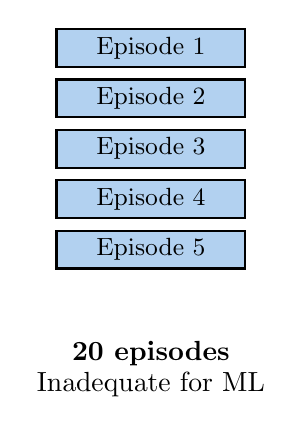
\begin{tikzpicture}[scale=0.8]
% Draw crisis episodes as blocks
\foreach \i in {1,...,5} {
    \draw[fill=maincolor!30, thick] (0, -\i*0.8) rectangle (3, -\i*0.8+0.6);
    \node at (1.5, -\i*0.8+0.3) {\small Episode \i};
}
\node[below] at (1.5, -5) {\textbf{20 episodes}};
\node[below] at (1.5, -5.5) {\alert{Inadequate for ML}};
\end{tikzpicture}
\end{center}
\end{columns}
\end{frame}

\begin{frame}{The Common Solution: Panel Expansion}
\begin{center}
\textbf{Transform each episode into daily observations}

\vspace{1em}
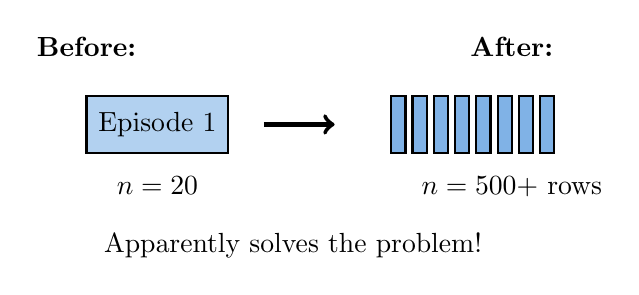
\begin{tikzpicture}[scale=0.9]
% Before
\node at (0, 2) {\textbf{Before:}};
\draw[fill=maincolor!30, thick] (0, 0.5) rectangle (2, 1.3);
\node at (1, 0.9) {Episode 1};
\node[below] at (1, 0.3) {$n = 20$};

% Arrow
\draw[->, ultra thick] (2.5, 0.9) -- (3.5, 0.9);

% After
\node at (6, 2) {\textbf{After:}};
\foreach \i in {1,...,8} {
    \draw[fill=maincolor!50, thick] (4+\i*0.3, 0.5) rectangle (4.2+\i*0.3, 1.3);
}
\node[below] at (6, 0.3) {$n = 500+$ rows};

\node[below, align=center] at (3, -0.5) {
    \alert{Apparently solves the problem!}
};
\end{tikzpicture}
\end{center}

\vspace{1em}
\begin{center}
\Large But first... what IS an episode?
\end{center}
\end{frame}

\begin{frame}{What is an Episode?}
\textbf{Episode = One independent case tracked over time}

\vspace{0.5em}
\begin{columns}[T]
\column{0.55\textwidth}
\structure{Geopolitics (this paper's context):}

\textbf{Episode = One country-crisis situation}
\begin{itemize}
\item \textbf{Episode 1: Venezuela 2017-2019}
  \begin{itemize}
  \item Day 0, 1, 2, ..., 45 $\to$ \alert{Coup attempt!}
  \end{itemize}
\item \textbf{Episode 2: Turkey 2015-2016}
  \begin{itemize}
  \item Day 0, 1, 2, ..., 120 $\to$ \alert{Coup attempt!}
  \end{itemize}
\item \textbf{Episode 3: Switzerland 2015-2020}
  \begin{itemize}
  \item Day 0, 1, 2, ..., 1825 $\to$ \structure{Stable}
  \end{itemize}
\end{itemize}

\vspace{0.3em}
\small Each country-crisis = one episode tracked daily

\column{0.4\textwidth}
\structure{Same concept applies to:}
\begin{itemize}
\item \textbf{Healthcare:} One patient
  \begin{itemize}
  \item ICU admission $\to$ death or discharge
  \end{itemize}
\item \textbf{Engineering:} One machine
  \begin{itemize}
  \item Installation $\to$ failure
  \end{itemize}
\item \textbf{Business:} One customer
  \begin{itemize}
  \item Sign-up $\to$ churn
  \end{itemize}
\end{itemize}
\end{columns}

\vspace{0.5em}
\begin{center}
\tikz{
    \node[draw, fill=maincolor!20, rounded corners, text width=0.85\textwidth, align=center, thick] {
        \textbf{Key:} Episodes are independent, but observations \\
        \textbf{within} the same episode are highly correlated!
    };
}
\end{center}
\end{frame}

\begin{frame}{Why Hazard Must Be Small for Rare Events}
\textbf{Question:} If events are rare, shouldn't the daily risk be very small?

\vspace{0.5em}
\structure{YES! Exactly right. Let's see why:}

\vspace{0.5em}
\textbf{Hazard} = Risk something happens \textbf{today} given it hasn't happened yet

\begin{columns}[T]
\column{0.48\textwidth}
\alert{If hazard is HIGH (say 50\%):}
\begin{itemize}
\item 50\% chance event happens today
\item 50\% chance tomorrow
\item 50\% chance next day...
\item Most episodes have events \alert{quickly}
\item \alert{NOT A RARE EVENT!}
\end{itemize}

\vspace{0.3em}
\begin{center}
\tikz{
    \node[draw, fill=red!20, rounded corners, text width=0.9\columnwidth, align=center] {
        High hazard $\to$ \\Common events
    };
}
\end{center}

\column{0.48\textwidth}
\structure{If hazard is LOW (say 5\%):}
\begin{itemize}
\item Only 5\% chance today
\item Only 5\% chance tomorrow
\item Only 5\% chance next day...
\item Most days: no event
\item \structure{TRULY RARE EVENT!}
\end{itemize}

\vspace{0.3em}
\begin{center}
\tikz{
    \node[draw, fill=green!20, rounded corners, text width=0.9\columnwidth, align=center] {
        Low hazard $\to$ \\Rare events
    };
}
\end{center}
\end{columns}

\vspace{0.5em}
\begin{center}
\textbf{This is why we use -3:} logit$^{-1}$(-3) $\approx$ 5\% daily hazard $\to$ truly rare!
\end{center}
\end{frame}

\begin{frame}{Visualizing Episodes Over Time}
\begin{center}
\textbf{Each episode is a time series:}

\vspace{0.5em}
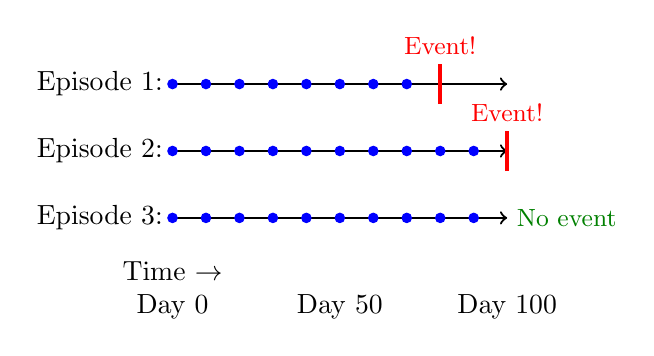
\begin{tikzpicture}[scale=0.85]
% Episode 1
\draw[->, thick] (0,3) -- (5,3);
\node[left] at (0,3) {Episode 1:};
\foreach \x in {0,0.5,1,1.5,2,2.5,3,3.5} {
    \filldraw[blue] (\x,3) circle (2pt);
}
\draw[red, ultra thick] (4,2.7) -- (4,3.3);
\node[above, red] at (4,3.3) {\small Event!};

% Episode 2
\draw[->, thick] (0,2) -- (5,2);
\node[left] at (0,2) {Episode 2:};
\foreach \x in {0,0.5,1,1.5,2,2.5,3,3.5,4,4.5} {
    \filldraw[blue] (\x,2) circle (2pt);
}
\draw[red, ultra thick] (5,1.7) -- (5,2.3);
\node[above, red] at (5,2.3) {\small Event!};

% Episode 3
\draw[->, thick] (0,1) -- (5,1);
\node[left] at (0,1) {Episode 3:};
\foreach \x in {0,0.5,1,1.5,2,2.5,3,3.5,4,4.5} {
    \filldraw[blue] (\x,1) circle (2pt);
}
\node[right, green!50!black] at (5,1) {\small No event};

% Time axis
\node[below] at (0,0.5) {Time $\to$};
\node[below] at (0,0) {Day 0};
\node[below] at (2.5,0) {Day 50};
\node[below] at (5,0) {Day 100};
\end{tikzpicture}
\end{center}

\vspace{0.5em}
\textbf{Critical insight:}
\begin{itemize}
\item Points within same episode (blue dots close together) are \alert{correlated}
\item Points across episodes (Episode 1 vs Episode 2) are \structure{independent}
\item Standard CV ignores this structure!
\end{itemize}
\end{frame}

\section{Two Failure Modes}

\begin{frame}{Two Silent Failures}
\begin{columns}[T]
\column{0.48\textwidth}
\begin{block}{Failure \#1: Label Leakage}
Features that depend on $T_e$ create target leakage
\[X_{e,t} = f(T_e - t) + \epsilon\]
\textbf{Known problem} (Kaufman et al. 2012)
\end{block}

\column{0.48\textwidth}
\begin{block}{Failure \#2: Pseudoreplication}
Row-wise CV treats correlated observations as independent
\[\text{Same episode in train \& test}\]
\textbf{Our focus:} More dangerous than leakage!
\end{block}
\end{columns}

\vspace{2em}
\begin{center}
\Large\alert{But what exactly IS leakage?}\\[0.5em]
\large Let's understand both concepts before seeing the results...
\end{center}
\end{frame}

\begin{frame}{What is Data Leakage?}
\textbf{Simple definition:} Using information in training that won't be available when making real predictions

\vspace{1em}
\structure{The Time-Travel Problem:}

\begin{center}
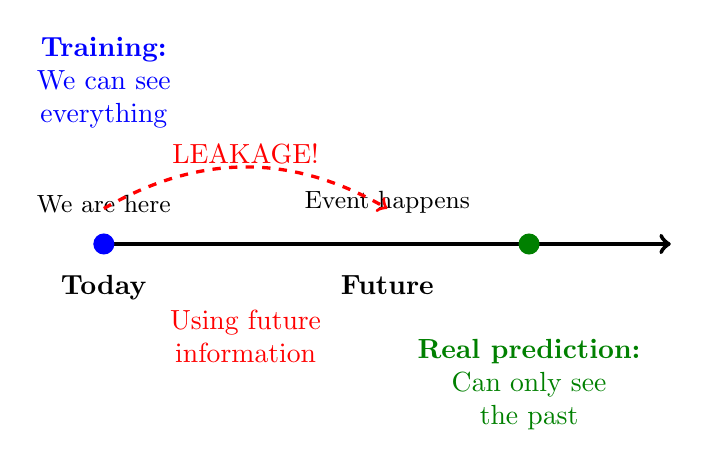
\begin{tikzpicture}[scale=0.9]
% Timeline
\draw[->, ultra thick] (0,0) -- (8,0);
\node[below] at (0,-0.3) {\textbf{Today}};
\node[below] at (4,-0.3) {\textbf{Future}};
\node[above] at (0,0.3) {\small We are here};
\node[above] at (4,0.3) {\small Event happens};

% Training phase
\filldraw[blue] (0,0) circle (4pt);
\node[above, blue, align=center] at (0,1.5) {\textbf{Training:}\\We can see\\everything};

% Leakage arrow
\draw[->, red, very thick, dashed] (0,0.5) to[bend left] (4,0.5);
\node[above, red] at (2,1) {\alert{LEAKAGE!}};
\node[below, red, align=center] at (2,-0.8) {Using future\\information};

% Real prediction
\filldraw[green!50!black] (6,0) circle (4pt);
\node[below, green!50!black, align=center] at (6,-1.2) {\textbf{Real prediction:}\\Can only see\\the past};
\end{tikzpicture}
\end{center}

\vspace{0.5em}
\textbf{Result:} Model looks great in training, fails in deployment!
\end{frame}

\begin{frame}{Temporal Label Leakage: The Core Idea}
\textbf{In forecasting, leakage means using information that depends on the future event time}

\vspace{1em}
\begin{columns}[T]
\column{0.48\textwidth}
\structure{Valid Feature (No Leakage):}
\begin{itemize}
\item ``Protest count last week''
\item ``GDP growth last quarter''
\item ``Patient temperature yesterday''
\item ``Sensor reading 1 hour ago''
\end{itemize}

\vspace{0.5em}
\tikz{
    \node[draw, fill=goodcolor!20, rounded corners, text width=0.9\columnwidth, align=center] {
        Available BEFORE we need to predict
    };
}

\column{0.48\textwidth}
\alert{Leaked Feature (CHEATING):}
\begin{itemize}
\item ``Days until coup'' ($T_e - t$)
\item ``Time to patient death''
\item ``Hours until failure''
\item ``Weeks until churn''
\end{itemize}

\vspace{0.5em}
\tikz{
    \node[draw, fill=alertcolor!20, rounded corners, text width=0.9\columnwidth, align=center] {
        Only known AFTER the event!
    };
}
\end{columns}
\end{frame}

\begin{frame}{Example: Predicting Equipment Failure}
\textbf{Scenario:} Predict if machine will fail in next 7 days

\vspace{0.5em}
\begin{center}
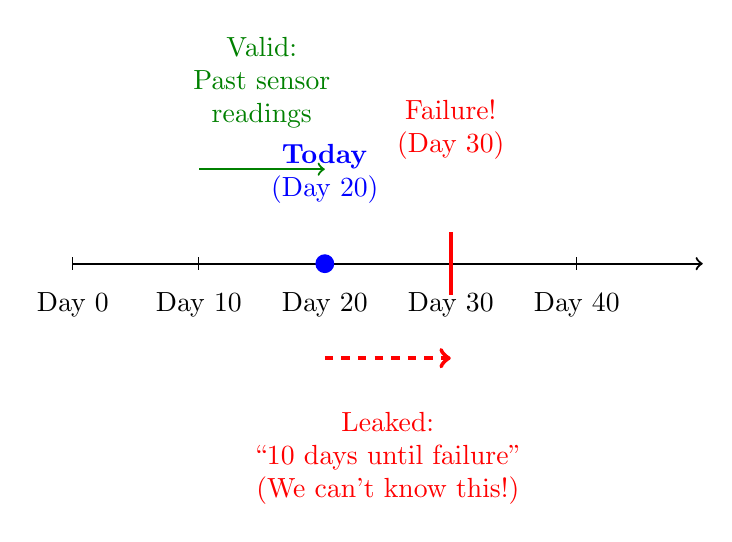
\begin{tikzpicture}[scale=0.8]
% Timeline
\draw[->, thick] (0,0) -- (10,0);
\foreach \x in {0,2,4,6,8} {
    \draw (\x,0.1) -- (\x,-0.1);
}
\node[below] at (0,-0.3) {Day 0};
\node[below] at (2,-0.3) {Day 10};
\node[below] at (4,-0.3) {Day 20};
\node[below] at (6,-0.3) {Day 30};
\node[below] at (8,-0.3) {Day 40};

% Current time
\filldraw[blue] (4,0) circle (4pt);
\node[above, blue, align=center] at (4,0.8) {\textbf{Today}\\(Day 20)};

% Failure time
\draw[red, ultra thick] (6,-0.5) -- (6,0.5);
\node[above, red, align=center] at (6,1.5) {\alert{Failure!}\\(Day 30)};

% Valid features
\draw[<-, green!50!black, thick] (4,1.5) -- (2,1.5);
\node[above, green!50!black, align=center] at (3,2) {\structure{Valid:}\\Past sensor\\readings};

% Leaked feature
\draw[->, red, ultra thick, dashed] (4,-1.5) -- (6,-1.5);
\node[below, red, align=center] at (5,-2.2) {\alert{Leaked:}\\``10 days until failure''\\(We can't know this!)};
\end{tikzpicture}
\end{center}

\vspace{0.5em}
\textbf{The Problem:}
\begin{itemize}
\item Feature: \alert{``Days until failure = 10''}
\item This is PERFECT information... but we can't have it!
\item In real deployment: We don't know when failure will occur
\end{itemize}
\end{frame}

\begin{frame}{Why Leakage is SO Dangerous}
\begin{enumerate}
\item \textbf{Creates perfect-looking models}
\begin{itemize}
\item AUC $>$ 0.95, Accuracy $>$ 95\%
\item Looks like you solved the problem!
\end{itemize}

\vspace{0.5em}
\item \textbf{Fails completely in deployment}
\begin{itemize}
\item Real-world performance: no better than random
\item The leaked feature doesn't exist at prediction time
\end{itemize}

\vspace{0.5em}
\item \textbf{Hard to detect}
\begin{itemize}
\item Implicit leakage (global normalization, means)
\item Future information hidden in preprocessing
\item Can slip through code review
\end{itemize}

\vspace{0.5em}
\item \textbf{Wastes resources}
\begin{itemize}
\item Deploy a system that doesn't work
\item Lose trust from stakeholders
\item Months of work thrown away
\end{itemize}
\end{enumerate}
\end{frame}

\begin{frame}{Our Contribution}
\textbf{This paper makes four key contributions:}

\vspace{1em}
\begin{enumerate}
\item \structure{Novel empirical finding:}
\begin{itemize}
\item \alert{Pseudoreplication (+54\%) is the dominant threat}
\item Exceeds even explicit time-to-event leakage (+39\%)
\item Challenges conventional focus on feature-level leakage
\end{itemize}

\vspace{0.5em}
\item \structure{Unified framework:}
\begin{itemize}
\item First to formalize \textit{both} failure modes together
\item Show how they interact in panel-expanded forecasting
\item Provide solutions for both
\end{itemize}

\vspace{0.5em}
\item \structure{Simple diagnostic ($\Delta_{\text{CV}}$):}
\begin{itemize}
\item Detects pseudoreplication: gap between random and grouped CV
\item No new data needed - just re-run evaluation
\item In our simulation: $\Delta_{\text{CV}} = 0.30$ (severe!)
\end{itemize}

\vspace{0.5em}
\item \structure{Corrected protocol:}
\begin{itemize}
\item Episode-grouped evaluation (fixes pseudoreplication)
\item Feature audit (fixes leakage)
\item Cluster-aware uncertainty (fixes both)
\end{itemize}
\end{enumerate}
\end{frame}





\begin{frame}{Research Question}
\begin{center}
\LARGE
\textbf{In panel-expanded rare-event forecasting,}\\[0.5em]
\textbf{which failure mode dominates?}

\vspace{1em}
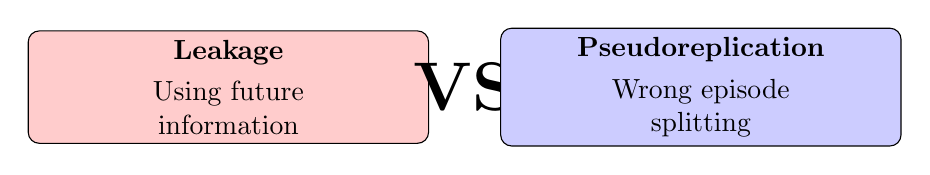
\begin{tikzpicture}
\node[draw, fill=red!20, rounded corners, text width=0.4\textwidth, align=center] at (0,0) {
    \textbf{Leakage}\\[0.3em]
    Using future\\information
};

\node at (3,0) {\Huge \textbf{VS}};

\node[draw, fill=blue!20, rounded corners, text width=0.4\textwidth, align=center] at (6,0) {
    \textbf{Pseudoreplication}\\[0.3em]
    Wrong episode\\splitting
};
\end{tikzpicture}

\vspace{2em}
\large
\structure{Spoiler:} It's not the one everyone worries about: Tests pseudoreplication...
\end{center}
\end{frame}



\begin{frame}{Our Key Finding: The Standard Tool Is Worse}
\textbf{Which is more dangerous?}

\vspace{1em}
\begin{columns}[T]
\column{0.48\textwidth}
\structure{Explicit Leakage:}

\texttt{df['days\_until'] =} \\
\texttt{~~T\_e - t}

\vspace{0.5em}
\begin{itemize}
\item Obviously wrong
\item Everyone catches it
\item Code review flags it
\item \alert{Inflation: +39\%}
\end{itemize}

\vspace{0.5em}
\begin{center}
\tikz{
    \node[draw, fill=red!20, rounded corners, text width=0.8\columnwidth, align=center] {
        Visible threat\\Easy to detect
    };
}
\end{center}

\column{0.48\textwidth}
\structure{Standard K-Fold CV:}

\texttt{from sklearn import KFold} \\
\texttt{cv = KFold(5)}

\vspace{0.5em}
\begin{itemize}
\item Looks completely safe
\item Default in docs
\item Passes all checks
\item \alert{Inflation: +54\%}
\end{itemize}

\vspace{0.5em}
\begin{center}
\tikz{
    \node[draw, fill=orange!40, rounded corners, text width=0.8\columnwidth, align=center] {
        \textbf{Invisible threat}\\
        \textbf{MORE dangerous!}
    };
}
\end{center}
\end{columns}

\vspace{1em}
\begin{center}
\Large
\alert{The default tool causes 54\% inflation vs. 39\% for explicit cheating!}
\end{center}
\end{frame}




\begin{frame}{What is Pseudoreplication?}
\textbf{Definition:} Treating observations as independent when they're actually correlated

\vspace{1em}
\structure{The term comes from ecology (Hurlbert 1984):}

\begin{center}
\begin{tikzpicture}[scale=0.8]
% Two ponds
\draw[thick, fill=blue!10] (0,0) ellipse (1.5 and 1);
\node[above] at (0,1.2) {\textbf{Pond A}};
\node[above] at (0,0.8) {\small (treated)};

\draw[thick, fill=blue!10] (4,0) ellipse (1.5 and 1);
\node[above] at (4,1.2) {\textbf{Pond B}};
\node[above] at (4,0.8) {\small (control)};

% Fish in Pond A
\foreach \i in {1,2,3,4,5} {
    \node at (0, -0.5+\i*0.2) {��};
}

% Fish in Pond B
\foreach \i in {1,2,3,4,5} {
    \node at (4, -0.5+\i*0.2) {��};
}

% Labels
\node[below] at (0,-1.5) {\alert{5 fish from same pond}};
\node[below] at (4,-1.5) {\alert{5 fish from same pond}};
\end{tikzpicture}
\end{center}

\vspace{0.5em}
\textbf{WRONG:} Claim $n=10$ independent samples

\textbf{RIGHT:} Only $n=2$ independent samples (2 ponds)

\vspace{0.5em}
\alert{Fish within same pond share water quality, temperature, food → correlated!}
\end{frame}

\begin{frame}{Pseudoreplication in Panel Data}
\textbf{Same problem happens with time-indexed panels!}

\vspace{1em}
\begin{columns}[T]
\column{0.48\textwidth}
\structure{The Setup:}
\begin{itemize}
\item 30 episodes (countries)
\item Each tracked for $\sim$30 days
\item Total: 900 rows
\end{itemize}

\vspace{0.5em}
\textbf{WRONG claim:} $n=900$ independent samples!

\vspace{0.5em}
\textbf{Reality:}
\begin{itemize}
\item Days within same country are correlated
\item Venezuela Day 5 $\approx$ Venezuela Day 6
\item Same geopolitical context
\item Same underlying risk factors
\end{itemize}

\column{0.48\textwidth}
\structure{The Math:}

With intraclass correlation $\rho$ and $m$ observations per episode:

\[n_{\text{eff}} = \frac{n}{1 + (m-1)\rho}\]

\vspace{0.5em}
\textbf{Example:} $m=30$ days, $\rho=0.5$

\[n_{\text{eff}} = \frac{900}{1 + 29 \times 0.5} = \frac{900}{15.5} \approx 58\]

\vspace{0.5em}
\alert{15$\times$ reduction!}

\vspace{0.5em}
True sample size: Only 58, not 900!
\end{columns}
\end{frame}

\begin{frame}{Why Standard CV Fails}
\textbf{Standard K-Fold CV ignores episode structure:}

\vspace{1em}
\begin{center}
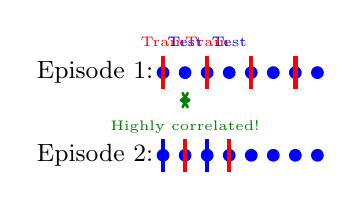
\begin{tikzpicture}[scale=0.7]
% Episode 1
\node[left] at (0,3) {\small Episode 1:};
\foreach \x in {0,0.4,0.8,1.2,1.6,2.0,2.4,2.8} {
    \filldraw[blue] (\x,3) circle (3pt);
}

% Show train/test split
\draw[red, ultra thick] (0,2.7) -- (0,3.3);
\draw[red, ultra thick] (0.8,2.7) -- (0.8,3.3);
\draw[red, ultra thick] (1.6,2.7) -- (1.6,3.3);
\draw[red, ultra thick] (2.4,2.7) -- (2.4,3.3);

\node[above, red] at (0,3.3) {\tiny Train};
\node[above, blue] at (0.4,3.3) {\tiny Test};
\node[above, red] at (0.8,3.3) {\tiny Train};
\node[above, blue] at (1.2,3.3) {\tiny Test};

% Arrow showing correlation
\draw[<->, green!50!black, very thick] (0.3,2.5) -- (0.5,2.5);
\node[below, green!50!black] at (0.4,2.3) {\tiny Highly correlated!};

% Episode 2
\node[left] at (0,1.5) {\small Episode 2:};
\foreach \x in {0,0.4,0.8,1.2,1.6,2.0,2.4,2.8} {
    \filldraw[blue] (\x,1.5) circle (3pt);
}

% Train/test split
\draw[blue, ultra thick] (0,1.2) -- (0,1.8);
\draw[red, ultra thick] (0.4,1.2) -- (0.4,1.8);
\draw[blue, ultra thick] (0.8,1.2) -- (0.8,1.8);
\draw[red, ultra thick] (1.2,1.2) -- (1.2,1.8);
\end{tikzpicture}
\end{center}

\vspace{0.5em}
\textbf{The Problem:}
\begin{enumerate}
\item Train on Venezuela Day 5
\item Test on Venezuela Day 6
\item Model sees: ``Ah, this looks like Venezuela!''
\item Predicts based on episode identity, not actual risk
\end{enumerate}

\vspace{0.5em}
\alert{This is CHEATING - model memorizes episodes instead of learning patterns!}
\end{frame}


\section{Episode Memorization}

\begin{frame}{The Mechanism: Episode Memorization}
\textbf{What standard K-Fold CV does:}
\begin{enumerate}
\item Randomly assigns \alert{rows} to folds
\item Episode $e$ appears in \alert{both} training and test
\item Consecutive observations $X_{e,t}$ and $X_{e,t+1}$ highly correlated
\end{enumerate}

\vspace{1em}
\textbf{What the model learns:}
\begin{itemize}
\item Not: ``What patterns precede events?''
\item But: \alert{``Which episode does this belong to?''}
\item Identity inference → pattern matching → artificial accuracy
\end{itemize}

\vspace{1em}
\begin{center}
\tikz{
    \node[draw, fill=alertcolor!20, rounded corners, text width=0.7\textwidth, align=center] {
        \textbf{Forecasting} (extrapolation to new episodes)\\
        transforms into\\
        \textbf{Interpolation} (pattern-matching within known episodes)
    };
}
\end{center}
\end{frame}

\begin{frame}{Visualizing the Problem}
\begin{columns}[T]
\column{0.48\textwidth}
\textbf{Standard K-Fold (WRONG):}
\begin{center}
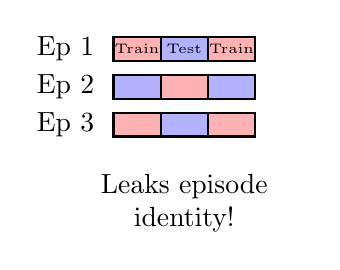
\begin{tikzpicture}[scale=0.6]
% Episode 1 split across folds
\draw[fill=red!30, thick] (0, 3) rectangle (1, 3.5);
\node at (0.5, 3.25) {\tiny Train};
\draw[fill=blue!30, thick] (1, 3) rectangle (2, 3.5);
\node at (1.5, 3.25) {\tiny Test};
\draw[fill=red!30, thick] (2, 3) rectangle (3, 3.5);
\node at (2.5, 3.25) {\tiny Train};
\node[left] at (-0.2, 3.25) {Ep 1};

% Episode 2 split
\draw[fill=blue!30, thick] (0, 2.2) rectangle (1, 2.7);
\draw[fill=red!30, thick] (1, 2.2) rectangle (2, 2.7);
\draw[fill=blue!30, thick] (2, 2.2) rectangle (3, 2.7);
\node[left] at (-0.2, 2.45) {Ep 2};

% Episode 3 split
\draw[fill=red!30, thick] (0, 1.4) rectangle (1, 1.9);
\draw[fill=blue!30, thick] (1, 1.4) rectangle (2, 1.9);
\draw[fill=red!30, thick] (2, 1.4) rectangle (3, 1.9);
\node[left] at (-0.2, 1.65) {Ep 3};

\node[below, align=center, text width=3cm] at (1.5, 0.8) {
    \alert{Leaks episode identity!}
};
\end{tikzpicture}
\end{center}

\column{0.48\textwidth}
\textbf{Episode-Grouped (CORRECT):}
\begin{center}
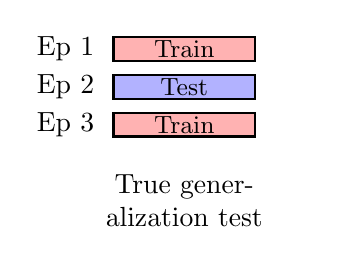
\begin{tikzpicture}[scale=0.6]
% Episode 1 all in train
\draw[fill=red!30, thick] (0, 3) rectangle (3, 3.5);
\node at (1.5, 3.25) {\small Train};
\node[left] at (-0.2, 3.25) {Ep 1};

% Episode 2 all in test
\draw[fill=blue!30, thick] (0, 2.2) rectangle (3, 2.7);
\node at (1.5, 2.45) {\small Test};
\node[left] at (-0.2, 2.45) {Ep 2};

% Episode 3 all in train
\draw[fill=red!30, thick] (0, 1.4) rectangle (3, 1.9);
\node at (1.5, 1.65) {\small Train};
\node[left] at (-0.2, 1.65) {Ep 3};

\node[below, align=center, text width=3cm] at (1.5, 0.8) {
    \structure{True generalization test}
};
\end{tikzpicture}
\end{center}
\end{columns}
\end{frame}

\section{Simulation}

\begin{frame}{Understanding the Hazard Function}
\textbf{What is a hazard?}

Think of it as: \structure{"What's the probability an event happens TODAY, given it hasn't happened yet?"}

\vspace{1em}
\begin{columns}[T]
\column{0.48\textwidth}
\textbf{Examples:}
\begin{itemize}
\item Probability of coup \alert{today} given no coup yet
\item Probability of equipment failure \alert{today} given still working
\item Probability patient deteriorates \alert{today} given stable so far
\end{itemize}

\column{0.48\textwidth}
\begin{center}
\begin{tikzpicture}[scale=0.7]
% Timeline
\draw[->, thick] (0,0) -- (5,0);
\foreach \x in {0,1,2,3,4} {
    \draw (\x,0.1) -- (\x,-0.1);
    \node[below] at (\x,-0.2) {\tiny Day \x};
}
% Show hazard at each day
\foreach \x in {0,1,2,3} {
    \draw[->, red, thick] (\x+0.5,0) -- (\x+0.5,0.8);
    \node[above, red] at (\x+0.5,0.8) {\tiny $h_t$};
}
\node[below, align=center] at (2.5,-1) {
    \structure{Each day has its own\\hazard probability}
};
\end{tikzpicture}
\end{center}
\end{columns}
\end{frame}

\begin{frame}{Our Hazard Function: Building Blocks}
\[\alert{h_{e,t}} = \text{logit}^{-1}(\structure{-3} + \structure{\alpha_e} + \structure{0.15 \cdot Z_{e,t}})\]

\textbf{Let's break this down piece by piece:}

\vspace{0.5em}
\begin{enumerate}
\item \structure{$\alpha_e$} = Episode-specific baseline risk
\begin{itemize}
\item Some countries/patients/machines are just riskier than others
\item Example: Venezuela vs. Switzerland have different coup risks
\item Drawn from $\mathcal{N}(0, 0.5)$ → some high, some low
\end{itemize}

\vspace{0.3em}
\item \structure{$Z_{e,t}$} = Time-varying risk signal
\begin{itemize}
\item Evolves day-by-day: $Z_{e,t} = 0.7 Z_{e,t-1} + \text{noise}$
\item \alert{0.7 = autocorrelation} → today's risk similar to yesterday's
\item This is what creates the "texture" models memorize!
\end{itemize}
\end{enumerate}
\end{frame}

\begin{frame}{Hazard Function: The Critical Parameters}
\[\alert{h_{e,t}} = \text{logit}^{-1}(\structure{-3} + \alpha_e + \structure{0.15} \cdot Z_{e,t})\]

\begin{enumerate}
\setcounter{enumi}{2}
\item \structure{0.15} = Signal strength (intentionally weak!)
\begin{itemize}
\item Controls how much $Z_{e,t}$ affects risk
\item Small value (0.15) → hard prediction problem
\item Makes baseline model weak (AUC = 0.56)
\end{itemize}

\vspace{0.3em}
\item \structure{-3} = \alert{The intercept (MOST IMPORTANT!)}
\begin{itemize}
\item Controls base event rate
\item $\text{logit}^{-1}(-3) \approx 0.047 = 5\%$
\item \alert{This makes events truly rare!}
\end{itemize}
\end{enumerate}

\vspace{0.5em}
\begin{center}
\tikz{
    \node[draw, fill=maincolor!20, rounded corners, text width=0.8\textwidth, align=center, thick] {
        \textbf{Key insight:} Without the -3, events would happen 50\% of the time\\
        (not rare at all!). The -3 creates the problem we're studying.
    };
}
\end{center}
\end{frame}

\begin{frame}{Why -3? A Visual Explanation}
\textbf{The logit$^{-1}$ (sigmoid) function converts numbers to probabilities:}

\vspace{0.5em}
\begin{center}
\begin{tikzpicture}[scale=0.9]
% Draw sigmoid curve
\draw[->] (-4,0) -- (4,0) node[right] {Input};
\draw[->] (0,0) -- (0,4) node[above] {Probability};

% Draw curve
\draw[very thick, blue, domain=-4:4, samples=100] plot (\x, {3/(1+exp(-1.5*\x))});

% Mark key points
\filldraw[red] (-3, 3/(1+exp(4.5))) circle (3pt);
\draw[red, dashed] (-3, 0) -- (-3, 3/(1+exp(4.5))) -- (0, 3/(1+exp(4.5)));
\node[below, red] at (-3, 0) {$-3$};
\node[left, red] at (0, 3/(1+exp(4.5))) {$\sim$5\%};

\filldraw[green!50!black] (0, 1.5) circle (3pt);
\draw[green!50!black, dashed] (0, 0) -- (0, 1.5) -- (-0.5, 1.5);
\node[below, green!50!black] at (0, 0) {$0$};
\node[left, green!50!black] at (-0.5, 1.5) {50\%};

\filldraw[orange] (3, 3/(1+exp(-4.5))) circle (3pt);
\draw[orange, dashed] (3, 0) -- (3, 3/(1+exp(-4.5))) -- (0, 3/(1+exp(-4.5)));
\node[below, orange] at (3, 0) {$+3$};
\node[left, orange] at (0, 3/(1+exp(-4.5))) {$\sim$95\%};
\end{tikzpicture}
\end{center}

\begin{itemize}
\item Input = 0 → 50\% probability (balanced, \alert{not rare})
\item Input = -3 → \structure{5\% probability (truly rare!)}
\item Input = +3 → 95\% probability (very common)
\end{itemize}
\end{frame}

\begin{frame}{Simulation Setup: Putting It All Together}
\textbf{Goal:} Create realistic rare-event forecasting scenario

\vspace{0.5em}
\textbf{Design:} $E = 30$ episodes (countries, patients, machines) with:

\begin{enumerate}
\item Each episode gets a baseline risk: $\alpha_e \sim \mathcal{N}(0, 0.5)$
\begin{itemize}
\item Some inherently riskier than others
\end{itemize}

\vspace{0.3em}
\item Day-by-day risk evolves: $Z_{e,t} = 0.7 Z_{e,t-1} + \epsilon_t$
\begin{itemize}
\item Autocorrelated (today $\approx$ yesterday)
\item This autocorrelation is what models memorize!
\end{itemize}

\vspace{0.3em}
\item Calculate daily hazard: $h_{e,t} = \text{logit}^{-1}(-3 + \alpha_e + 0.15 Z_{e,t})$
\begin{itemize}
\item Average daily event rate $\approx$ 5\%
\item Weak signal (0.15) → hard problem
\end{itemize}

\vspace{0.3em}
\item Features: Built from past $Z$ values only (no cheating!)
\item Label: Did event occur in next 14 days?
\end{enumerate}
\end{frame}

\begin{frame}{Four Test Conditions}
\textbf{We test each failure mode independently:}

\vspace{1em}
\begin{enumerate}
\item \structure{Leak-free + Grouped CV} \hfill (\structure{Baseline - correct!})
\begin{itemize}
\item Features from past only, proper episode splitting
\item This is how it \alert{should} be done
\end{itemize}

\vspace{0.3em}
\item \alert{Leak-free + Random CV} \hfill (\alert{Pseudoreplication test})
\begin{itemize}
\item Same clean features, but wrong CV
\item Tests: How much does default KFold hurt?
\end{itemize}

\vspace{0.3em}
\item Normalization leak + Grouped CV
\begin{itemize}
\item Tests implicit leakage from global statistics
\end{itemize}

\vspace{0.3em}
\item \alert{Explicit leak + Grouped CV} \hfill (\alert{Leakage test})
\begin{itemize}
\item Features include $T_e - t$ (days until event)
\item Tests: How much does worst leakage hurt?
\end{itemize}
\end{enumerate}
\end{frame}

\section{Main Result}

\begin{frame}{The Main Finding}
\begin{center}
\LARGE\structure{Pseudoreplication > Leakage}

\vspace{2em}
\begin{tabular}{lcc}
\toprule
\textbf{Failure Mode} & \textbf{AUC Inflation} & \textbf{Relative} \\
\midrule
\alert{Pseudoreplication} & 0.56 → 0.86 & \alert{+54\%} \\
Explicit Leakage & 0.56 → 0.77 & +39\% \\
\bottomrule
\end{tabular}

\vspace{2em}
\Large
\alert{The standard tool is more dangerous}\\
\alert{than the worst feature-engineering error!}
\end{center}
\end{frame}

\begin{frame}{Detailed Results}
\begin{table}
\centering
\small
\begin{tabular}{lccc}
\toprule
\textbf{Condition} & \textbf{AUC} & \textbf{Brier} & \textbf{Inflation} \\
\midrule
Leak-Free + Grouped CV & 0.56 $\pm$ 0.07 & 0.29 $\pm$ 0.05 & baseline \\
\rowcolor{red!10}
Leak-Free + Random CV & \textbf{0.86 $\pm$ 0.04} & 0.15 $\pm$ 0.02 & \alert{+54\%} \\
Norm. Leak + Grouped & 0.56 $\pm$ 0.07 & 0.29 $\pm$ 0.05 & +0\%$^\dagger$ \\
Explicit Leak + Grouped & 0.77 $\pm$ 0.04 & 0.16 $\pm$ 0.03 & +39\% \\
\bottomrule
\end{tabular}
\end{table}

\vspace{0.5em}
\footnotesize
$^\dagger$Normalization leak requires pre-existing trends; our AR(1) features are stationary (conservative design)

\vspace{1em}
\textbf{Key insight:} Autocorrelation alone (no trends, no leakage) destroys validity
\end{frame}

\begin{frame}{Why Pseudoreplication Dominates}
\begin{columns}[T]
\column{0.48\textwidth}
\textbf{Leakage:}
\begin{itemize}
\item Requires specific conditions
\item Explicit $T_e - t$ features
\item OR trending features + global normalization
\item \structure{Visible in code review}
\end{itemize}

\column{0.48\textwidth}
\textbf{Pseudoreplication:}
\begin{itemize}
\item Requires \alert{only default KFold}
\item Single line of code everyone uses
\item \alert{Invisible and ubiquitous}
\item \alert{Activated by default}
\end{itemize}
\end{columns}

\vspace{2em}
\begin{center}
\tikz{
    \node[draw, fill=alertcolor!20, rounded corners, text width=0.8\textwidth, align=center, thick] {
        \textbf{Asymmetry:} Leakage is rare and detectable.\\
        Pseudoreplication is \alert{everywhere} and invisible.
    };
}
\end{center}
\end{frame}

\begin{frame}{Performance Decouples from Sample Size}
\begin{center}
\structure{Under random CV, performance ignores effective $n$:}

\vspace{0.5em}

\includegraphics[width=0.7\textwidth]{figs/figure1_simulation_results.png}

\vspace{0.5em}
\small
Panel D shows: Model achieves AUC $> 0.8$ even when $n_{\text{eff}} < 50$\\
\alert{→ Exploiting autocorrelation artifact, not learning generalizable signal}
\end{center}
\end{frame}

\section{The Solution}

\begin{frame}{The $\Delta_{\text{CV}}$ Diagnostic}
\textbf{Simple check for episode memorization:}
\[\Delta_{\text{CV}} := \widehat{\text{AUC}}_{\text{random}} - \widehat{\text{AUC}}_{\text{grouped}}\]

\vspace{1em}
\textbf{Interpretation:}
\begin{itemize}
\item $\Delta_{\text{CV}} < 0.05$: Model is okay
\item $\Delta_{\text{CV}} > 0.05$: \alert{Model relies on episode memorization}
\item $\Delta_{\text{CV}} > 0.10$: \alert{\textbf{Severe problem}}
\end{itemize}

\vspace{1em}
\textbf{In our simulation:} $\Delta_{\text{CV}} = 0.30$ (catastrophic!)

\vspace{1em}
\structure{Requires no new data—just re-run with GroupKFold}
\end{frame}

\begin{frame}{Corrected Protocol}
\begin{enumerate}
\item \textbf{Preprocessing:}
\begin{itemize}
\item Fit transformations on training fold only
\item Forward-fill imputation (not mean)
\item Trailing windows (not centered)
\end{itemize}

\vspace{0.5em}
\item \textbf{Evaluation:}
\begin{itemize}
\item Use \texttt{GroupKFold} with \texttt{groups=episode\_id}
\item \alert{Never split episodes across folds}
\end{itemize}

\vspace{0.5em}
\item \textbf{Reporting:}
\begin{itemize}
\item Report $\Delta_{\text{CV}}$ alongside AUC
\item Report $n_{\text{eff}}$ (effective sample size)
\item Brier Score and Log Loss as primary metrics
\end{itemize}
\end{enumerate}
\end{frame}

\begin{frame}{Red Flags}
\begin{center}
\Large\alert{Warning signs that should trigger audits:}

\vspace{1em}
\begin{tabular}{ll}
\toprule
\textbf{Metric} & \textbf{Threshold} \\
\midrule
AUC & $> 0.85$ with $E < 50$ episodes \\
$\Delta_{\text{CV}}$ & $> 0.10$ \\
Brier Score & $< 0.10$ on imbalanced data \\
\bottomrule
\end{tabular}

\vspace{2em}
\structure{If you see performance this good on rare events...}\\
\structure{...it's probably too good to be true!}
\end{center}
\end{frame}

\section{Implications}

\begin{frame}{Affected Domains}
\textbf{This pathology affects any field using panel-expanded forecasting:}

\vspace{0.5em}
\begin{columns}[T]
\column{0.48\textwidth}
\begin{itemize}
\item \structure{Geopolitics:} Conflict forecasting, coups
\item \structure{Healthcare:} Clinical deterioration, mortality
\item \structure{Engineering:} Predictive maintenance, equipment failure
\end{itemize}

\column{0.48\textwidth}
\begin{itemize}
\item \structure{Business:} Customer churn, default prediction
\item \structure{Finance:} Credit events, bankruptcy
\item \structure{Any rare event} expanded into daily/hourly panels
\end{itemize}
\end{columns}

\vspace{1em}
\begin{center}
\tikz{
    \node[draw, fill=maincolor!20, rounded corners, text width=0.9\textwidth, align=center, thick] {
        \textbf{Call for Action:} Retrospective audits of published claims\\
        in rare-event forecasting using panel data
    };
}
\end{center}
\end{frame}

\begin{frame}{Relation to Prior Work}
\textbf{We unify three research streams:}

\vspace{0.5em}
\begin{enumerate}
\item \textbf{Kaufman et al. (2012):} Leakage formalization, learn-predict separation
\begin{itemize}
\item But: focused on i.i.d. data, explicit violations
\end{itemize}

\vspace{0.3em}
\item \textbf{Roberts et al. (2017):} Block CV for structured data
\begin{itemize}
\item But: spatial dependence in ecology, not temporal panels
\end{itemize}

\vspace{0.3em}
\item \textbf{Hurlbert (1984):} Pseudoreplication in experiments
\begin{itemize}
\item But: experimental design, not ML evaluation
\end{itemize}
\end{enumerate}

\vspace{1em}
\structure{Our contribution:} Pseudoreplication \alert{dominates} in panel forecasting + $\Delta_{\text{CV}}$ diagnostic
\end{frame}

\section{Conclusion}

\begin{frame}{Key Takeaways}
\begin{enumerate}
\item Panel expansion creates value \alert{only if evaluation respects episode boundaries}

\vspace{0.5em}
\item Standard K-Fold CV—\alert{the default in Scikit-Learn}—violates this

\vspace{0.5em}
\item Result: \alert{Episode memorization} inflates AUC by 54\%

\vspace{0.5em}
\item This \alert{exceeds explicit leakage} (+39\%)

\vspace{0.5em}
\item The $\Delta_{\text{CV}}$ diagnostic provides a simple check

\vspace{0.5em}
\item \textbf{Action:} Use \texttt{GroupKFold}, report $\Delta_{\text{CV}}$ and $n_{\text{eff}}$
\end{enumerate}
\end{frame}

\begin{frame}{The Bottom Line}
\begin{center}
\LARGE
\alert{The standard tool is more dangerous}\\[0.3em]
\alert{than the worst feature-engineering error}

\vspace{2em}
\Large
\structure{Pseudoreplication is:}
\begin{itemize}
\item Invisible
\item Ubiquitous  
\item Activated by default
\item More impactful than explicit leakage
\end{itemize}

\vspace{1em}
\normalsize
\textbf{For reviewers:} Demand grouped CV, $\Delta_{\text{CV}}$ reporting, and $n_{\text{eff}}$ disclosure
\end{center}
\end{frame}

\begin{frame}[standout]
\begin{center}
\LARGE
Thank you!

\vspace{2em}
\normalsize
\textbf{Behnaz Moradi-Jamei}\\
moradibx@jmu.edu

\vspace{0.5em}
\textbf{Heman Shakeri}\\
hs@virginia.edu

\vspace{2em}
\structure{Code \& Materials:}\\
\texttt{github.com/[your-repo]}
\end{center}
\end{frame}

\appendix

\begin{frame}[allowframebreaks]{Backup: Effective Sample Size}
\textbf{Under intraclass correlation $\rho$ with $m$ observations per episode:}
\[n_{\text{eff}} = \frac{n}{1 + (m-1)\rho}\]

\vspace{1em}
\textbf{Example:} $n = 600$, $m = 20$, $\rho = 0.5$
\[n_{\text{eff}} = \frac{600}{1 + 19 \times 0.5} = \frac{600}{10.5} \approx 55\]

\vspace{1em}
\alert{10× reduction in effective sample size!}

\vspace{1em}
But pseudoreplication inflation is \textbf{not} just a sample-size effect—even with $n_{\text{eff}} < 20$, random CV achieves AUC $> 0.8$.
\end{frame}

\begin{frame}[allowframebreaks]{Backup: Why -3 Intercept?}
\textbf{Hazard function:} $h_{e,t} = \text{logit}^{-1}(-3 + \alpha_e + 0.15 Z_{e,t})$

\vspace{0.5em}
\textbf{Why the -3?}
\begin{itemize}
\item For average episode ($\alpha_e = 0$, $Z_{e,t} = 0$):
\[h_t = \text{logit}^{-1}(-3) = \frac{1}{1 + e^3} \approx 0.047 \approx 5\%\]

\item Creates \alert{truly rare events} (5\% base rate)
\item Matches empirical geopolitical event frequencies
\item Produces severe EPV constraint (EPV $< 5$)
\end{itemize}

\vspace{0.5em}
\textbf{Without -3:} Events would occur $\sim$50\% of the time (not rare!)
\end{frame}

\end{document}
